\documentclass[10pt]{exam}
\usepackage[hon]{template-for-exam}
\usepackage{enumitem,multicol,multirow,tikz,fancybox,graphicx}
\usetikzlibrary{shadings,decorations.pathmorphing,arrows.meta,patterns,calc}
\setlist[enumerate,itemize]{topsep=0pt,itemsep=-1ex,partopsep=1ex,parsep=1ex}
\graphicspath{{./figures}}
\usepackage[export]{adjustbox}

\title{Motion Graph Stations}
\author{Rohrbach}
\date{\today}

\newcommand{\drawgraph}[2]{
        \draw[->,very thick] (0,#2) +(0,-2.2) -- +(0,2.2)
          node[midway, above, sloped, fill=white] 
          {#1};
        \draw[->,very thick] (0,#2) -- +(15,0) 
          node[midway, below] {Time};
        \draw[gray,thin,dotted,shift={(0,#2)}] 
          (0,-2) grid[step=0.5] ++(14.5,4);
        \draw[gray,shift={(0,#2)}] 
          (0,-2) grid[step=2] ++(14.5,4);
    }
      
\newcommand{\twographs}{
    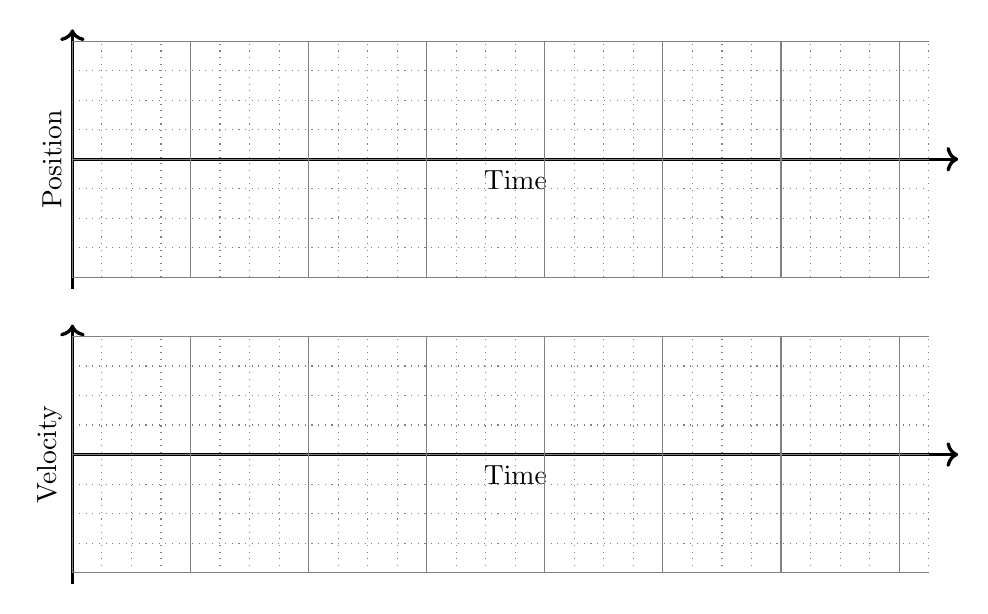
\begin{tikzpicture}[scale=0.75]
      \drawgraph{Position}{0}
      \drawgraph{Velocity}{-5}
    \end{tikzpicture}
}

\begin{document}
\maketitle

\noindent
\emph{\small Stations 1-2 are based off of Experiment \#2 in} Physics with Vernier\emph{, and the images have been taken from there.}

\section{Cart on an Incline}

\begin{center}
  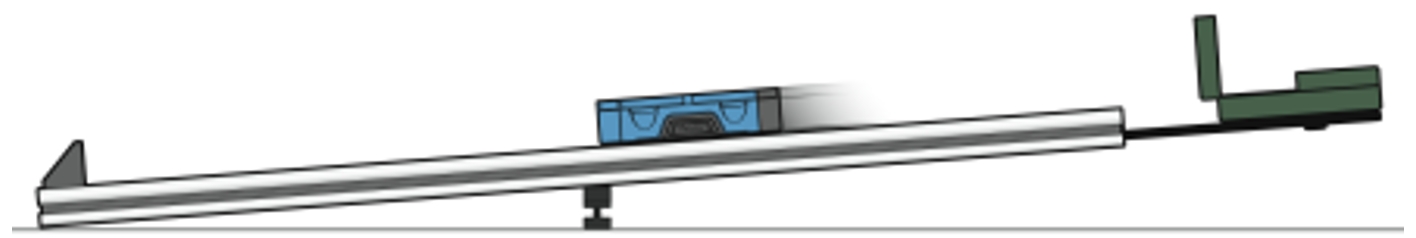
\includegraphics[width=4in]{incline.png}
\end{center}

\begin{enumerate}
  
  \item Place the cart on the track near the bottom. Press the play button to start data collection and then give the cart a push up the incline. Let the cart roll freely up nearly to the top, and then back down. Keep your hands away from the track as the cart rolls, then catch the cart as it nears the end stop. The cart should not get closer than 0.15 m to the motion detector. If you do not see a smooth graph, the cart was most likely not in the beam of the motion detector. Make adjustments and repeat data collection until you get a smooth graph.
  \item Sketch the position and velocity graphs below.  Please \textbf{be careful} with the horizontal axis.  Try to make it so that each graph has the same events occuring at the same location along the $t$-axis.  Don't rush this step.

  \twographs

  \item Was the acceleration constant or changing? How can you tell? \vs 
  \item Was there any point in the motion where the velocity was zero? Explain. \vs
  \item Was there any point in the motion where the acceleration was zero? Explain. \vs

\end{enumerate}


\section{Pendulum}

\begin{center}
  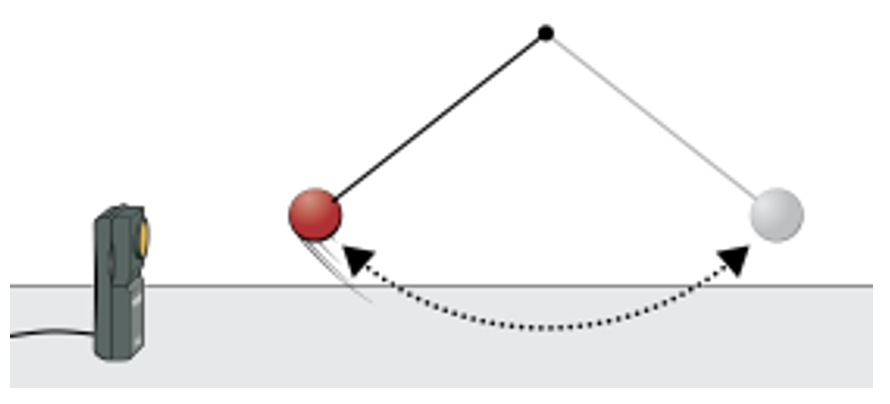
\includegraphics[width=2.7in]{pend.png}
\end{center}

\begin{enumerate}
  \item Place the motion detector near the pendulum. The motion detector should be level with, and about 1~m away from, the pendulum bob when it hangs at rest. The bob should never be closer to the detector than 25~cm.  Pull the pendulum about 15~cm toward the motion detector and release it to start the pendulum swinging.
  \item Press play to start data collection.
  \item When data collection is complete, a graph of position vs. time is displayed. If you do not see a smooth graph, the pendulum was most likely not in the beam of the motion detector. Make adjustments and repeat until you get a smooth graph.
  \item  Sketch the position and velocity graphs below.  Please \textbf{be careful} with the horizontal axis.  Try to make it so that each graph has the same events occuring at the same location along the $t$-axis.  Don't rush this step.

  \twographs

  \item Was the acceleration constant or changing? How can you tell? \vs
  \item Was there any point in the motion where the velocity was zero? Explain. \vs 
  \item Was there any point in the motion where the acceleration was zero? Explain. \vs 
  \item Where was the pendulum bob when the acceleration was greatest? \vs 


\end{enumerate}


\section{Bouncing Basketball}

\begin{enumerate}
  \item  Hold the basketball about 50 cm away from the motion detector.  Start taking data, and then drop the ball, allowing it to bounce a few times.
  \item See if your data looks smooth.  If there have been issues, take a new data set before proceeding.
  \item  Sketch the position and velocity graphs below.  Please \textbf{be careful} with the horizontal axis.  Try to make it so that each graph has the same events occuring at the same location along the $t$-axis.  Don't rush this step.

  \twographs

  \item Was there any point in the motion where the acceleration was constant? Explain. \vs 

  \item Was there any point in the motion where the velocity was zero? Explain. \vs 

  \item Why were there ``breaks'' in the velocity graph where the data jumped from negative to positive?  What happened at these locations? \vs
\end{enumerate}

\pagebreak

\section{Graph Match}

\emph{\small This station is based off of Experiment \#1 in} Physics with Vernier\emph{, and the images have been taken from there.}

\begin{center}
  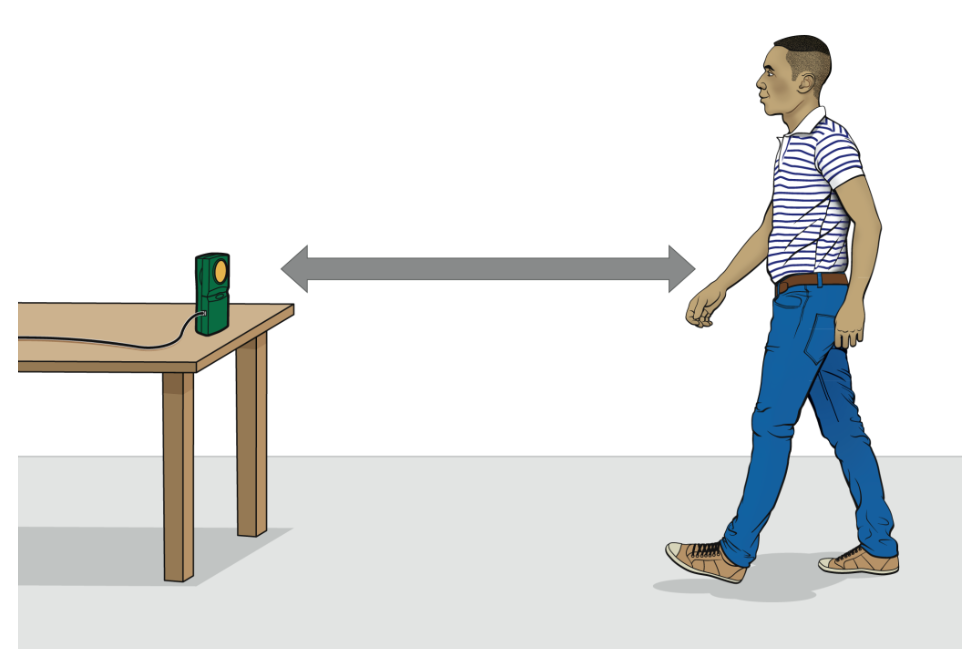
\includegraphics[width=2in]{walking.png}
  
\end{center}

\begin{multicols}{2}

\subsection*{Setup}
\begin{enumerate}
  \item Connect the motion detector to your computer. %Launch \texttt{Graphical Analysis}.

  \item Download \texttt{graph-match.gambl} from Schoology and open it in \texttt{Graphical Analysis}.

  %\item Place the motion detector so that it points toward an open space at least 2 m long. Use short strips of masking tape on the floor to mark distances of 0.5 m, 1 m, 1.5 m, and 2 m from the motion detector.  
  %Set the switch on your motion detector should be set to Ball/Walk. 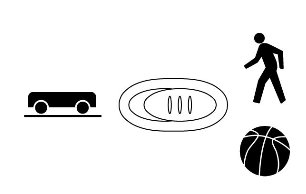
\includegraphics[height=2em,valign=t]{switch}
  %\item If two graphs are displayed, click or tap View, 
\includegraphics[height=1.2em]{view}, and choose 1 Graph (a graph of a position vs. time should be displayed).

  \item Find the position on the ground marked ``0 meters'' and stand there.  Have a lab partner Zero the sensor by [... FINISH ...]


  \item Monitor the position readings and practice walking toward the motion detector. Sometimes you will have to walk backwards. Confirm that the position values make sense as you move back and forth. 

\end{enumerate}


\subsection*{Position vs. Time Matching}\begin{enumerate}[resume]
  \item Click or tap Graph Tools, 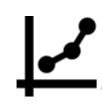
\includegraphics[height=1.2em]{graph-tools}, and choose Add Graph Match. Choose Position. A position target graph is displayed for you to match.
  \item Think about how you would walk to reproduce the target graph.  To test your prediction, choose a starting position. Start data collection, then walk in such a way that the graph of your motion matches the target graph on the screen.
  \item If you were not successful, start data collection again when you are ready to begin walking. Repeat this process until your motion closely matches the graph on the screen.
  \item Have every member of your group try. To perform a second position graph match, click or tap Graph Tools, 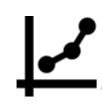
\includegraphics[height=1.2em]{graph-tools}, choose Add Graph Match, and then Position.
\end{enumerate}

\subsection*{Velocity vs. Time Matching}\begin{enumerate}[resume]
  \item \texttt{Graphical Analysis} can also generate random target velocity graphs for you to match. Click or tap Graph Tools,  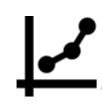
\includegraphics[height=1.2em]{graph-tools}, and choose Add Graph Match. Choose Velocity to view a velocity target graph. 
  \item Try to reproduce the target graph.  Keep repeating until you get something that closely matches.
  \item Repeat for every member of your group.  %To perform a second velocity graph match, click or tap Graph Tools, 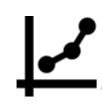
\includegraphics[height=1.2em]{graph-tools}, choose Add Graph Match, and then Velocity.
\end{enumerate}

\end{multicols}


\subsection*{Analysis}

\begin{enumerate}
  \item Explain the significance of the slope of a position vs. time graph. Include a discussion of positive and negative slope. \vs 
  \item What type of motion is occurring when the slope of a position vs. time graph is zero? \vs
  \item What type of motion is occurring when the slope of a position vs. time graph is constant? \vs
  \item What type of motion is occurring when the slope of a velocity vs. time graph is zero? \vs
\end{enumerate}
 


\end{document}